\RequirePackage[T1]{fontenc}   % before the class, so IEEEtran's Times (ptm) loads in T1
\documentclass[conference]{IEEEtran}
\IEEEoverridecommandlockouts
\usepackage[utf8]{inputenc}
\renewcommand{\ttdefault}{lmtt}   % Latin Modern Typewriter for code-like names
\usepackage[spanish,es-nodecimaldot,es-tabla,es-noshorthands]{babel}
\usepackage{cite}
\usepackage{amsmath,amssymb}
\usepackage{graphicx}
\usepackage{booktabs}
\usepackage{array}
\usepackage{textcomp}
\usepackage{xcolor}
\usepackage{microtype}
\usepackage[hidelinks]{hyperref}
\usepackage{url}
\def\UrlBreaks{\do\_\do\.\do\/\do\-}

\newcommand{\x}{\ensuremath{\times}}
\makeatletter\newcommand{\tabinput}[1]{\@@input #1 }\makeatother   % TeX primitive: works inside tabular with booktabs rules
\newcolumntype{L}[1]{>{\raggedright\arraybackslash}p{#1}}
\renewcommand{\figurename}{Figura}
\renewcommand{\IEEEkeywordsname}{Palabras clave}

\begin{document}

\title{Orquestador de \textit{swarms} de agentes LLM agnóstico al modelo y al dominio
\thanks{Paper, curso Inteligencia Artificial (G1), Universidad Icesi, Cali, Colombia. Versión 2.1, 12 de octubre de 2026.}}

\author{\IEEEauthorblockN{Julián Andrés Mendoza Castro}
\IEEEauthorblockA{Código A00395237\\
Universidad Icesi\\
Cali, Colombia\\
1109185879@u.icesi.edu.co}
\and
\IEEEauthorblockN{Esteban Gaviria Zambrano}
\IEEEauthorblockA{Código A00396019\\
Universidad Icesi\\
Cali, Colombia\\
esteban.gaviria@u.icesi.edu.co}}

\maketitle

\begin{abstract}
Un \textit{swarm} de agentes LLM reparte una tarea entre varios agentes que se comunican, y cada agente y cada mensaje consumen cómputo. Este trabajo presenta un orquestador reina--obreros que cambia de modelo y de dominio solo con configuración y lo usa para responder cuándo coordinar compensa su costo. Para que un \textit{swarm} tuviera margen de mejorar, se usaron modelos pequeños que se equivocan con frecuencia: dos pares fuerte/débil (Qwen 2.5 de 3B/1.5B y Llama 3.2 de 3B/1B), ejecutados al 100\,\% en una misma GPU de 4\,GB. Se compararon \textit{swarms} jerárquicos y en malla con 2 y 4 obreros, con reina débil o fuerte, frente al agente único fuerte, al débil y a la votación por mayoría con el mismo número de llamadas, en GSM8K-Platinum, MATH-500 nivel~5 y un plan de viaje a Cartagena. En 3\,640 corridas con hipótesis registradas de antemano, los \textit{swarms} costaron entre 1.8\x{} y 20.7\x{} los GPU-segundos del agente débil, y la energía siguió a los GPU-segundos. Los \textit{swarms} formados solo por el modelo débil no mejoraron al agente débil y quedaron por debajo de la votación en GSM8K (de $-0.08$ a $-0.19$). Con reina fuerte quedaron por debajo del modelo fuerte solo (de $-0.07$ a $-0.23$), a un costo de 2.4\x{} a 12.0\x{}. Cambiar solo la reina por el modelo fuerte sí mejoró la exactitud en GSM8K (de $+0.11$ a $+0.19$) y redujo los planes inválidos de Llama del 81--92\,\% al 22--39\,\% de las corridas. Con modelos pequeños, el cuello de botella es la coordinación: conviene un mejor coordinador o un modelo más capaz, no más agentes.
\end{abstract}

\begin{IEEEkeywords}
Sistemas multiagente, modelos de lenguaje, orquestación, costo--calidad, votación por mayoría, modelos locales, energía.
\end{IEEEkeywords}

\section{Introducción}

Los sistemas multiagente basados en LLM asignan roles a varios agentes que conversan para resolver una tarea \cite{guo2024survey}. AutoGen los modela como conversaciones programables \cite{wu2024autogen}, GPTSwarm como grafos optimizables \cite{zhuge2024gptswarm}, y herramientas como Ruflo los ofrecen como \textit{swarms} con una reina y obreros \cite{ruflo}. Coordinar tiene un costo directo: Anthropic reporta que su sistema de investigación multiagente usa unas 15 veces los tokens de un chat \cite{anthropic2025multiagent}. También tiene un costo de fiabilidad: la taxonomía MAST atribuye la mayoría de los fallos de estos sistemas al diseño y a la coordinación \cite{cemri2025mast}. Además, cuando el agente único ya resuelve más del 45\,\% de una tarea, agregar agentes da retornos negativos \cite{kim2025scaling}.

La pregunta de este trabajo es la que plantea la retroalimentación del curso: \emph{¿agregar agentes y comunicación mejora la calidad lo suficiente para justificar el aumento de costo?} Un primer estudio nuestro con un modelo de API (\texttt{deepseek-flash}) no pudo responderla. El agente único resolvió el 100\,\% de las tareas, así que solo podía mostrarse que coordinar cuesta más \cite{repo2026swarm}. Este trabajo cambia el diseño para que un \textit{swarm} tenga margen de mejorar. Las contribuciones son cuatro:
\begin{itemize}
\item Un orquestador reina--obreros en Python, agnóstico al modelo y al dominio, publicado con todos sus registros \cite{repo2026swarm}.
\item Un diseño de pares de capacidad con modelos locales, 100\,\% en GPU, que mide el cómputo (GPU-segundos) y la energía de cada llamada.
\item Una comparación contra la línea base que suele faltar: la votación por mayoría del modelo débil con el mismo número de llamadas \cite{wang2023selfconsistency,li2024moreagents}. La comparación usa hipótesis registradas antes de ejecutar y pruebas pareadas con corrección de Holm \cite{holm1979}.
\item Evidencia de que, con modelos pequeños, la ganancia viene de la reina y no del número de obreros.
\end{itemize}

\section{Trabajo relacionado}

La Tabla~\ref{tab:rel} ubica este trabajo. AutoGen reportó que su conversación multiagente supera a GPT-4 solo en MATH \cite{wu2024autogen}. AgentPrune muestra que muchas aristas de comunicación sobran \cite{zhang2025agentprune}, y MacNet escala la colaboración a más de mil agentes \cite{qian2025macnet}. Para un solo modelo, muestrear varias respuestas y votar mejora con el número de muestras \cite{wang2023selfconsistency,li2024moreagents}. Por el teorema del jurado de Condorcet \cite{condorcet1785}, la votación funciona mejor cuanto más independientes son los errores, pero los errores de los LLM están correlacionados \cite{kim2025correlated}. Kim et~al.~\cite{kim2025scaling} miden además que los sistemas multiagente amplifican los errores frente al agente único. Kapoor et~al.~\cite{kapoor2024agents} piden comparar agentes siempre contra su costo y contra líneas base simples. Este trabajo sigue esa recomendación con topologías fijas y cómputo medido en hardware.

\begin{table}[t]
\centering
\caption{Trabajos relacionados y lo que mide cada uno}
\label{tab:rel}
\footnotesize
\setlength{\tabcolsep}{3pt}
\begin{tabular}{@{}L{1.9cm}L{2.4cm}L{3.6cm}@{}}
\toprule
Trabajo & Organización & Qué mide \\
\midrule
AutoGen \cite{wu2024autogen} & conversación entre agentes & exactitud (MATH, otras) \\
GPTSwarm \cite{zhuge2024gptswarm} & grafo optimizable & exactitud y costo de optimizar \\
AgentPrune \cite{zhang2025agentprune} & poda de aristas & tokens frente a exactitud \\
Votación \cite{wang2023selfconsistency,li2024moreagents} & muestras independientes & exactitud frente a número de muestras \\
MAST \cite{cemri2025mast} & 7 marcos existentes & 14 modos de fallo \\
Kim et~al. \cite{kim2025scaling} & 5 arquitecturas & escalamiento y amplificación de errores \\
Este trabajo & único, jerárquica, malla; reina débil o fuerte & exactitud, GPU-segundos y energía frente a votación con igual número de llamadas \\
\bottomrule
\end{tabular}
\end{table}

\section{Metodología}

\subsection{Orquestador y topologías}

Un agente es un rol, unas instrucciones y un acceso a un LLM a través de una interfaz única, \texttt{LLM.complete()}, que oculta el proveedor. Las topologías (Fig.~\ref{fig:topo}) comparten cuatro etapas:
\begin{enumerate}
\item \textbf{Plan.} La reina reparte la tarea en una lista JSON con una subtarea por obrero. Si el JSON es inválido o no asigna una subtarea a cada obrero, se registra el fallo y cada obrero recibe la tarea completa.
\item \textbf{Trabajo.} Cada obrero resuelve su subtarea.
\item \textbf{Revisión} (solo en la malla). Cada obrero lee los borradores de todos y revisa el suyo.
\item \textbf{Integración.} La reina combina las contribuciones en la respuesta final.
\end{enumerate}
El agente único responde directamente con el mismo formato final. En los dominios matemáticos, los obreros cierran con una línea \texttt{\#\#\#\# <número>}. Así se sabe si algún obrero acertó y si la reina conservó la respuesta correcta.

\begin{figure}[t]
\centering
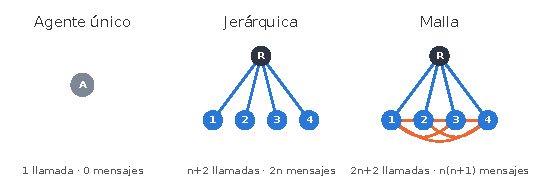
\includegraphics[width=\columnwidth]{figs/topologias.pdf}
\caption{Topologías con $n=4$ obreros. R es la reina; en la malla, las aristas naranjas forman la ronda de revisión entre obreros.}
\label{fig:topo}
\end{figure}

\subsection{Diseño: pares de capacidad y líneas base}

Cada familia aporta un modelo fuerte y uno débil: Qwen~2.5 de 3B y 1.5B \cite{qwen2025} y Llama~3.2 de 3B y 1B \cite{llama2024}, servidos con Ollama \cite{ollama}. Un \textit{swarm débil} usa el modelo débil en todos los agentes. Un \textit{swarm mixto} usa el fuerte solo en la reina. Ambos se ejecutan en topología jerárquica y en malla con $n\in\{2,4\}$ obreros. Las líneas base son el agente único fuerte, el agente único débil y la \textit{votación@k}: la respuesta más frecuente entre $k$ muestras independientes del modelo débil. La votación se empareja con cada \textit{swarm} por número de llamadas. La jerárquica con $n=2$ hace 4 llamadas y se compara con votación@3; la jerárquica con $n=4$ y la malla con $n=2$ hacen 6 y se comparan con votación@5; la malla con $n=4$ hace 10 y se compara con votación@9. Con $n$ obreros, la jerárquica hace $n+2$ llamadas e intercambia $2n$ mensajes, y la malla hace $2n+2$ llamadas y $n(n+1)$ mensajes. Si cada borrador mide $w$ tokens y el resto del \textit{prompt} $b$, la revisión de la malla lee
\begin{equation}
t^{\text{in}}_{\text{rev}}\approx n\,b+n^2 w
\label{eq:rev}
\end{equation}
tokens, así que su costo crece de forma cuadrática con $n$.

\subsection{Hipótesis registradas}

Antes de la primera corrida se fijaron ocho hipótesis y su prueba:
\begin{itemize}
\item \textbf{H1:} el costo crece con las llamadas y los mensajes.
\item \textbf{H2:} el \textit{swarm} débil cambia la exactitud del agente débil, en cualquier dirección.
\item \textbf{H3:} un \textit{swarm} supera a la votación con igual número de llamadas.
\item \textbf{H4:} el \textit{swarm} mixto alcanza al modelo fuerte solo.
\item \textbf{H5:} la reina fuerte reduce los fallos de coordinación.
\item \textbf{H6:} se describe cómo la reina conserva o pierde respuestas correctas.
\item \textbf{H7:} los errores del modelo débil están correlacionados.
\item \textbf{H8:} ambas familias ordenan igual las configuraciones.
\end{itemize}
También se fijó una regla de calibración. Un dominio es informativo para una familia si el agente débil resuelve entre el 10\,\% y el 90\,\% de 20 problemas de calibración, distintos de los de evaluación.

\subsection{Dominios}

La Tabla~\ref{tab:dom} resume los dominios. GSM8K-Platinum es la partición de prueba de GSM8K \cite{cobbe2021gsm8k} con las etiquetas erróneas corregidas \cite{vendrow2025platinum}. MATH-500 \cite{lightman2024verify} es un subconjunto de MATH \cite{hendrycks2021math}; se usaron problemas de nivel~5 con respuesta entera. La tarea abierta es el caso de Cartagena: un viaje de 3 días para un estudiante con 600\,000 COP. La calibración dejó GSM8K como informativo en ambas familias. MATH queda en nivel~5 porque la regla solo lo bajaba si ambas familias quedaban por debajo del 10\,\%, y solo Llama quedó en el piso (0\,\%). Por limitación de tiempo de cómputo, y antes de analizar resultados, MATH se redujo a 20 problemas con una repetición por \textit{swarm} (enmienda~B).

\begin{table}[t]
\centering
\caption{Dominios y calibración (exactitud del agente débil en 20 problemas de calibración)}
\label{tab:dom}
\footnotesize
\setlength{\tabcolsep}{3pt}
\begin{tabular}{@{}L{1.55cm}L{2.55cm}L{1.6cm}cc@{}}
\toprule
Dominio & Evaluación & Calidad & Qwen & Llama \\
\midrule
GSM8K-Platinum & 50 problemas; 2 rep. por \textit{swarm} & coincidencia exacta & 0.55 & 0.55 \\
MATH-500 niv.~5 & 20 problemas; 1 rep. por \textit{swarm} & coincidencia exacta & 0.15 & 0.00 \\
Cartagena & 1 plan; 2 rep. por configuración & rúbrica de 7 criterios & -- & -- \\
\bottomrule
\end{tabular}
\end{table}

\subsection{Protocolo y medición}

Cada modelo se verificó al 100\,\% en la VRAM de una RTX~3050 Laptop de 4\,GB, sin descarga a CPU, con ventana de 8\,192 tokens. Para que el modelo de 3B de Llama cupiera hizo falta \textit{flash attention} y una caché KV de 8 bits; sin ellas corría al 90\,\% en GPU. Se cargaba un solo modelo a la vez, se atendía una sola llamada a la vez, y el portátil estuvo conectado a la corriente en modo de rendimiento todo el experimento. Todas las configuraciones comparten temperatura 0.7, 1\,024 tokens máximos de salida y los mismos \textit{prompts}. El agente fuerte tiene 3 muestras por problema y el débil 9, de las que salen las votaciones. El cómputo de una corrida se mide en \textbf{GPU-segundos}: el tiempo de procesamiento del \textit{prompt} más el de generación que reporta Ollama. La \textbf{energía} es la integral de la potencia de la GPU muestreada a 20\,Hz por NVML. La potencia en reposo fue de 4.3\,W, y las cargas de modelo se registran aparte. Cada corrida tiene un identificador derivado de su especificación, se ejecuta en orden aleatorio con semilla fija y se puede reanudar.

\subsection{Evaluación y estadística}

En los dominios matemáticos, la calidad es la coincidencia exacta del número final. Cartagena se califica con una rúbrica de siete criterios binarios con reglas de decisión explícitas:
\begin{itemize}
\item itinerario por día;
\item presupuesto con total;
\item total dentro del límite;
\item alojamiento económico;
\item dos riesgos con su mitigación;
\item consistencia interna;
\item lugares concretos.
\end{itemize}
El plan registrado preveía dos evaluadores humanos. Por decisión de los autores, las 40 respuestas, exportadas sin modelo ni configuración y en orden aleatorio, las calificó a ciegas un evaluador LLM (Claude Opus 5.5) antes de abrir la clave (enmienda~C). \textbf{No es una evaluación humana} y tiene las limitaciones conocidas de los LLM como jueces \cite{zheng2023judging}. Las diferencias entre configuraciones se calculan por problema, emparejadas, con intervalos \textit{bootstrap} al 95\,\% y una prueba de permutación con cambio de signo. Las 80 comparaciones registradas se corrigen con Holm \cite{holm1979}.

\section{Resultados}

Se ejecutaron 3\,640 corridas de evaluación y 160 de calibración. Ninguna tuvo un fallo de infraestructura ni truncó el contexto; el \textit{prompt} más largo fue de 4\,281 tokens. La matriz completa tomó 10.0 horas de ejecución. La Tabla~\ref{tab:main} reúne la exactitud y el cómputo de todas las configuraciones.

\begin{table*}[t]
\centering
\caption{Exactitud (Ex.) y GPU-segundos por corrida (GPU-s) por familia y dominio, y puntaje de la rúbrica en Cartagena (evaluador LLM a ciegas). La votación@$k$ usa $k$ muestras del modelo débil. ``Jer'' es jerárquica; ``débil'' y ``mixto'' indican la reina débil o fuerte, con obreros siempre débiles.}
\label{tab:main}
\footnotesize
\setlength{\tabcolsep}{4.6pt}
\begin{tabular}{@{}lrrrrrrrrrr@{}}
\toprule
 & \multicolumn{2}{c}{Qwen, GSM8K} & \multicolumn{2}{c}{Llama, GSM8K} & \multicolumn{2}{c}{Qwen, MATH} & \multicolumn{2}{c}{Llama, MATH} & \multicolumn{2}{c}{Cartagena (rúbrica)} \\
\cmidrule(lr){2-3}\cmidrule(lr){4-5}\cmidrule(lr){6-7}\cmidrule(lr){8-9}\cmidrule(l){10-11}
Configuración & Ex. & GPU-s & Ex. & GPU-s & Ex. & GPU-s & Ex. & GPU-s & Qwen & Llama \\
\midrule
\tabinput{tabs/main.tex}
\bottomrule
\end{tabular}
\end{table*}

\subsection{Costo (H1)}

Las llamadas y los mensajes siguen las fórmulas de la sección anterior. Frente al agente débil, los \textit{swarms} usaron entre 1.8\x{} y 20.7\x{} los GPU-segundos en GSM8K y MATH, y hasta 26\x{} los tokens. En Cartagena usaron entre 3.4\x{} y 15.3\x{} los GPU-segundos. La malla con $n=4$ fue siempre la configuración más cara de su familia y equipo (Fig.~\ref{fig:cost}). La energía siguió a los GPU-segundos, con 55 a 73\,J por GPU-segundo en todas las configuraciones, así que el orden de costos es el mismo en ambas medidas. El costo es estructural: ambas familias ordenaron las configuraciones por costo casi igual (Kendall $\tau$ de 0.82 a 0.96, $p<0.001$).

\begin{figure*}[t]
\centering
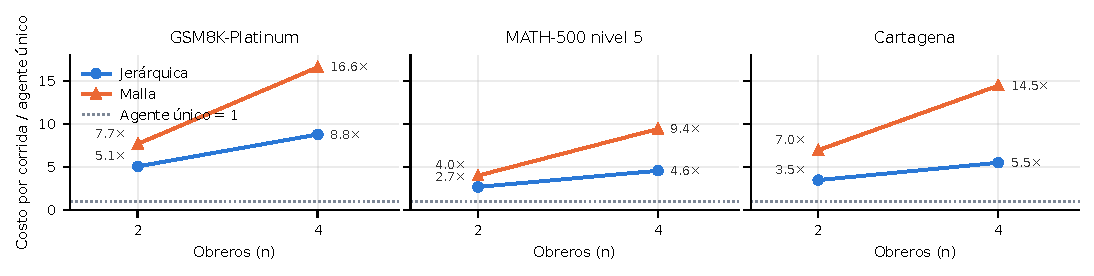
\includegraphics[width=\textwidth]{figs/costo_vs_n.pdf}
\caption{GPU-segundos por corrida relativos al agente único débil al pasar de $n=2$ a $n=4$ obreros. La línea punteada es el agente único fuerte. La malla (línea discontinua) crece más rápido que la jerárquica, y la reina fuerte añade costo.}
\label{fig:cost}
\end{figure*}

\subsection{Calidad frente a cómputo (H2--H4)}

La Fig.~\ref{fig:acc} pone cada configuración en el plano exactitud--cómputo, y la Tabla~\ref{tab:contr} resume las comparaciones registradas.
\begin{itemize}
\item \textbf{H2.} Ningún \textit{swarm} débil mejoró al agente débil en GSM8K, con diferencias de $-0.11$ a $-0.03$. En MATH con Qwen, tres de las cuatro formas sumaron $+0.11$, pero los intervalos incluyen el cero.
\item \textbf{H3.} Frente a la votación con el mismo número de llamadas, los \textit{swarms} débiles quedaron por debajo en GSM8K: de $-0.08$ a $-0.15$ con Qwen y de $-0.10$ a $-0.19$ con Llama. Seis de las ocho diferencias tienen $p<0.05$ sin corregir, pero ninguna sobrevive a Holm. Los \textit{swarms} mixtos empataron con la votación.
\item \textbf{H4.} El modelo fuerte solo fue mejor que cualquier \textit{swarm} mixto: de $0.07$ a $0.12$ puntos más con Qwen y de $0.20$ a $0.23$ con Llama, mientras los mixtos usaban entre 2.4\x{} y 5.9\x{} (Qwen) y entre 6.4\x{} y 12.0\x{} (Llama) sus GPU-segundos. Son las únicas diferencias significativas tras Holm: 3 de 80, todas de Llama en GSM8K, con $p_{\text{Holm}}$ entre 0.008 y 0.031.
\end{itemize}
En 4 de las 6 combinaciones de familia y dominio, la mejor configuración fue el agente único fuerte, con 1.5\x{} a 1.7\x{} el cómputo del débil. Las otras dos son Llama en MATH, en el piso (máximo 0.15), y Qwen en Cartagena (0.57 con dos respuestas por configuración); en ambas, un \textit{swarm} queda primero dentro del ruido.

\begin{figure*}[t]
\centering
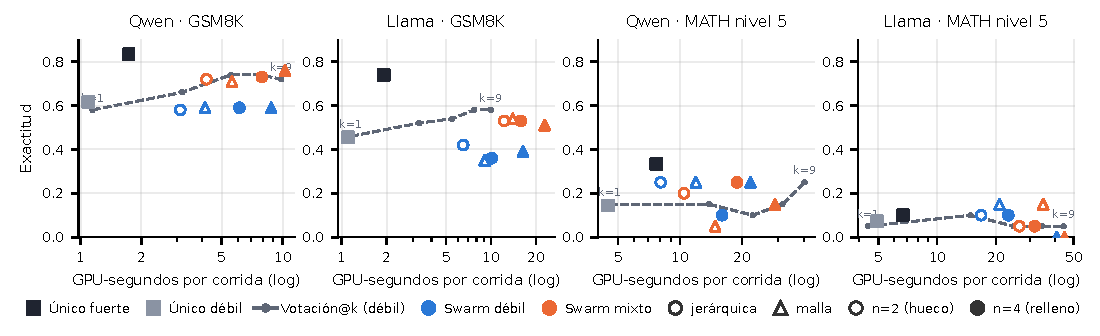
\includegraphics[width=\textwidth]{figs/exactitud_vs_gpu.pdf}
\caption{Exactitud frente a GPU-segundos por corrida (escala logarítmica). La línea discontinua es la votación del modelo débil con $k=1,3,5,7,9$ muestras. Los \textit{swarms} débiles (azul) quedan por debajo de esa curva y los mixtos (naranja) sobre ella, pero el agente único fuerte (cuadrado negro) los domina con menos cómputo.}
\label{fig:acc}
\end{figure*}

\begin{table}[t]
\centering
\caption{Diferencias de exactitud por problema (rango sobre las cuatro formas de \textit{swarm}), comparaciones con $p<0.05$ sin corregir y significativas tras Holm (de 80 en total)}
\label{tab:contr}
\scriptsize
\setlength{\tabcolsep}{1.6pt}
\resizebox{\columnwidth}{!}{%
\begin{tabular}{@{}lL{1.55cm}ccccrr@{}}
\toprule
 & Comparación & \multicolumn{2}{c}{GSM8K} & \multicolumn{2}{c}{MATH} & $p{<}.05$ & Holm \\
\cmidrule(lr){3-4}\cmidrule(lr){5-6}
 & & Qwen & Llama & Qwen & Llama & & \\
\midrule
\tabinput{tabs/contrasts.tex}
\bottomrule
\end{tabular}}
\end{table}

\subsection{Coordinación (H5, H6)}

El único cambio que mejoró la exactitud fue la reina. Con la misma forma y los mismos obreros débiles, la reina fuerte subió la exactitud en GSM8K de $+0.12$ a $+0.17$ con Qwen y de $+0.11$ a $+0.19$ con Llama (seis de ocho con $p\le 0.06$ sin corregir; ninguna tras Holm). El mecanismo difiere por familia (Tabla~\ref{tab:coord}, Fig.~\ref{fig:coord}):
\begin{itemize}
\item \textbf{Llama.} La reina de 1B produjo un plan inválido en el 81--92\,\% de las corridas, de modo que su \textit{swarm} débil mide sobre todo el modo de respaldo, en que cada obrero resuelve la tarea completa. Con reina de 3B, los planes inválidos bajaron al 22--39\,\%. Es el modo FM-1.1 de MAST, desobedecer la especificación \cite{cemri2025mast}.
\item \textbf{Qwen.} Los planes ya eran válidos, y la ganancia está en la integración: la reina fuerte conservó la respuesta correcta de un obrero en el 67--73\,\% de las corridas, frente al 53--58\,\% de la débil.
\end{itemize}
En GSM8K, la reina descartó la respuesta correcta de un obrero en el 3--29\,\% de las corridas. La revisión de la malla aumentó el número de obreros correctos en el 20--43\,\% de las corridas y lo redujo en el 8--21\,\%. La mejora interna existe, pero la integración no siempre la aprovecha.

\begin{table}[t]
\centering
\caption{Coordinación en GSM8K: fracción de corridas (rango sobre las cuatro formas) y modo MAST más cercano}
\label{tab:coord}
\scriptsize
\setlength{\tabcolsep}{2pt}
\begin{tabular}{@{}L{2.25cm}ccccL{1.2cm}@{}}
\toprule
 & \multicolumn{2}{c}{Qwen} & \multicolumn{2}{c}{Llama} & \\
\cmidrule(lr){2-3}\cmidrule(lr){4-5}
Evento & débil & mixto & débil & mixto & MAST \\
\midrule
\tabinput{tabs/coordination.tex}
\bottomrule
\end{tabular}
\end{table}

\begin{figure}[t]
\centering
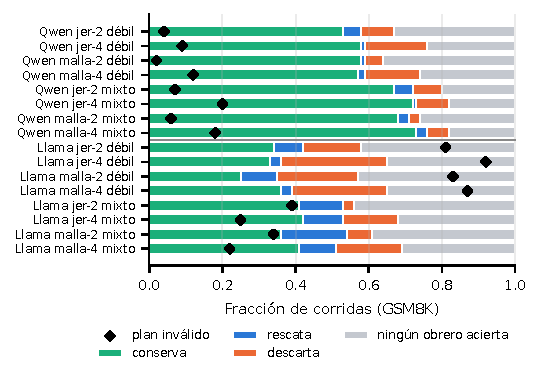
\includegraphics[width=\columnwidth]{figs/coordinacion.pdf}
\caption{Qué hizo la reina con la respuesta de los obreros en GSM8K, por configuración. Los rombos marcan la fracción de planes inválidos.}
\label{fig:coord}
\end{figure}

\subsection{Votación y correlación de errores (H7) y agnosticidad (H8)}

Las muestras del modelo débil cometen errores correlacionados: la correlación media entre pares de muestras fue de $\phi=0.24$ a $0.45$. Por eso la votación ayuda pero se estanca. En Qwen y GSM8K pasó de 0.62 a 0.74 con $k=5$ y bajó a 0.72 con $k=9$, por debajo del 0.77 que predice Condorcet con errores independientes. Cuando la exactitud individual es menor que 0.5, el modelo binario de Condorcet no sirve de referencia, porque las respuestas erróneas se reparten entre muchos números y la mayoría relativa aún acierta. En cuanto a la agnosticidad, ambas familias ordenaron igual las configuraciones por costo. Por calidad coincidieron en GSM8K ($\tau=0.58$, $p=0.023$), pero no en MATH ($\tau=-0.13$) ni en Cartagena ($\tau=0.15$).

\subsection{Cartagena}

Con la rúbrica, el agente único obtuvo 0.61 de media, la malla 0.48 y la jerárquica 0.39. Trece de las 40 respuestas llegaron al límite de 1\,024 tokens, casi todas de \textit{swarms}, y obtuvieron 0.40 frente a 0.51 de las completas. El límite era igual para todos, y truncar es otro costo de integrar más texto. Casi ninguna respuesta propuso dos riesgos con mitigación (1 de 40) o un presupuesto consistente (4 de 40), y los modelos de 1--3B cometieron errores de hecho sobre la ciudad. Con dos respuestas por configuración y un solo evaluador LLM, este resultado es descriptivo.

\section{Discusión}

La respuesta a la pregunta de investigación, con modelos de 1 a 3B, es negativa: agregar agentes y comunicación no compensó su costo. Hay dos alternativas más simples:
\begin{itemize}
\item Si hay un modelo más capaz disponible, usarlo solo fue mejor y entre 2.4\x{} y 12.0\x{} más barato que construir un \textit{swarm} alrededor de él.
\item Si solo hay un modelo débil, votar entre $k$ muestras fue al menos tan bueno como un \textit{swarm} con el mismo número de llamadas.
\end{itemize}
El resultado es coherente con Kim et~al.~\cite{kim2025scaling}: el agente débil resolvía el 46--62\,\% de GSM8K, por encima del umbral del 45\,\% donde agregar agentes deja de rendir.

Este estudio también muestra dónde está el problema. Los obreros acertaban con frecuencia, y la revisión de la malla los corregía. Lo que fallaba era la coordinación: planes que no seguían el formato y respuestas correctas descartadas al integrar. La única intervención que mejoró la exactitud fue darle a la reina un modelo más capaz. Para quien diseñe un \textit{swarm} con modelos pequeños, la implicación práctica es invertir el cómputo en el coordinador o en un modelo mejor, no en más obreros. Además, todo \textit{swarm} debería compararse contra la votación con el mismo número de llamadas.

Frente al primer estudio con \texttt{deepseek-flash}, la conclusión de que el agente único es la mejor opción se mantiene. Pero ahora no se debe a un efecto techo: los \textit{swarms} tenían margen para mejorar y no lo aprovecharon.

\section{Limitaciones y trabajo futuro}

\begin{itemize}
\item \textbf{Alcance de los modelos.} Solo se probaron modelos de 1 a 3B en una GPU de 4\,GB, con una temperatura y \textit{prompts} no ajustados por modelo. Modelos mayores o \textit{prompts} específicos podrían comportarse distinto.
\item \textbf{Muestras pequeñas.} Las muestras son de 50 y 20 problemas, así que la mayoría de las comparaciones tiene poca potencia, y Holm sobre 80 comparaciones es conservador. Llama en MATH está en el piso y aporta poca información.
\item \textbf{Modo de respaldo.} Cuando un plan es inválido, cada obrero recibe la tarea completa. Por eso el \textit{swarm} débil de Llama se parece a muestrear varias veces e integrar.
\item \textbf{Cartagena.} Es una sola tarea, con un evaluador LLM en lugar de dos humanos y respuestas truncadas en 1\,024 tokens.
\item \textbf{Energía.} Se midió solo la de la tarjeta gráfica.
\item \textbf{Contaminación.} GSM8K y MATH pueden estar en los datos de entrenamiento.
\end{itemize}
Como trabajo futuro proponemos:
\begin{itemize}
\item reinas especializadas o con salida estructurada forzada;
\item topologías podadas o adaptativas \cite{zhang2025agentprune,zhuge2024gptswarm};
\item tareas que se puedan descomponer de verdad;
\item evaluación humana con dos evaluadores.
\end{itemize}

\section{Conclusiones}

Se construyó un orquestador reina--obreros agnóstico al modelo y al dominio, y se midió en GPU cuánto cuesta y cuánto aporta coordinar modelos pequeños. En 3\,640 corridas, los \textit{swarms} costaron entre 1.8\x{} y 20.7\x{} el cómputo del agente débil y no superaron ni a la votación con el mismo número de llamadas ni al modelo fuerte solo. Lo que sí mejoró la exactitud fue cambiar la reina. Con modelos pequeños, la calidad de un \textit{swarm} depende de quién coordina más que de cuántos trabajan.

\section*{Disponibilidad de código y datos}
El código, los cuadernos ejecutados (V4.0, con la matriz completa, y V4.2, con el análisis), los registros de cada corrida, llamada y carga de modelo, la evaluación ciega de Cartagena y el script que genera las tablas y figuras de este artículo están en un repositorio público \cite{repo2026swarm}. El primer estudio con \texttt{deepseek-flash} queda archivado allí.

\begin{thebibliography}{99}

\bibitem{guo2024survey}
T.~Guo, X.~Chen, Y.~Wang, R.~Chang, S.~Pei, N.~V. Chawla, O.~Wiest, and X.~Zhang, ``Large language model based multi-agents: A survey of progress and challenges,'' arXiv:2402.01680, 2024.

\bibitem{wu2024autogen}
Q.~Wu, G.~Bansal, J.~Zhang \emph{et~al.}, ``AutoGen: Enabling next-gen LLM applications via multi-agent conversation,'' in \emph{Proc. Conf. Language Modeling (COLM)}, 2024. arXiv:2308.08155.

\bibitem{zhuge2024gptswarm}
M.~Zhuge, W.~Wang, L.~Kirsch, F.~Faccio, D.~Khizbullin, and J.~Schmidhuber, ``GPTSwarm: Language agents as optimizable graphs,'' in \emph{Proc. 41st Int. Conf. Machine Learning (ICML)}, PMLR 235, 2024.

\bibitem{ruflo}
ruvnet, ``Ruflo,'' repositorio de GitHub, 2026. \url{https://github.com/ruvnet/ruflo}

\bibitem{anthropic2025multiagent}
Anthropic, ``How we built our multi-agent research system,'' blog de ingeniería, 13 de junio de 2025. \url{https://www.anthropic.com/engineering/multi-agent-research-system}

\bibitem{cemri2025mast}
M.~Cemri, M.~Z. Pan, S.~Yang \emph{et~al.}, ``Why do multi-agent LLM systems fail?'' in \emph{Advances in Neural Information Processing Systems (NeurIPS), Datasets and Benchmarks Track}, 2025. arXiv:2503.13657.

\bibitem{kim2025scaling}
Y.~Kim, K.~Gu, C.~Park \emph{et~al.}, ``Towards a science of scaling agent systems,'' arXiv:2512.08296, 2025.

\bibitem{zhang2025agentprune}
G.~Zhang, Y.~Yue, Z.~Li, S.~Yun, G.~Wan, K.~Wang, D.~Cheng, J.~X. Yu, and T.~Chen, ``Cut the crap: An economical communication pipeline for LLM-based multi-agent systems,'' arXiv:2410.02506, 2024.

\bibitem{qian2025macnet}
C.~Qian, Z.~Xie, Y.~Wang \emph{et~al.}, ``Scaling large language model-based multi-agent collaboration,'' in \emph{Proc. Int. Conf. Learning Representations (ICLR)}, 2025.

\bibitem{wang2023selfconsistency}
X.~Wang, J.~Wei, D.~Schuurmans, Q.~Le, E.~Chi, S.~Narang, A.~Chowdhery, and D.~Zhou, ``Self-consistency improves chain of thought reasoning in language models,'' in \emph{Proc. Int. Conf. Learning Representations (ICLR)}, 2023.

\bibitem{li2024moreagents}
J.~Li, Q.~Zhang, Y.~Yu, Q.~Fu, and D.~Ye, ``More agents is all you need,'' \emph{Trans. Machine Learning Research (TMLR)}, 2024.

\bibitem{condorcet1785}
M.~J.~A.~N. de Caritat, marqués de Condorcet, \emph{Essai sur l'application de l'analyse à la probabilité des décisions rendues à la pluralité des voix}. París: Imprimerie Royale, 1785.

\bibitem{kim2025correlated}
E.~Kim, A.~Garg, K.~Peng, and N.~Garg, ``Correlated errors in large language models,'' in \emph{Proc. 42nd Int. Conf. Machine Learning (ICML)}, 2025.

\bibitem{kapoor2024agents}
S.~Kapoor, B.~Stroebl, Z.~S. Siegel, N.~Nadgir, and A.~Narayanan, ``AI agents that matter,'' arXiv:2407.01502, 2024.

\bibitem{holm1979}
S.~Holm, ``A simple sequentially rejective multiple test procedure,'' \emph{Scandinavian Journal of Statistics}, vol.~6, no.~2, pp.~65--70, 1979.

\bibitem{qwen2025}
Qwen Team, ``Qwen2.5 technical report,'' arXiv:2412.15115, 2024.

\bibitem{llama2024}
A.~Grattafiori, A.~Dubey, A.~Jauhri \emph{et~al.}, ``The Llama 3 herd of models,'' arXiv:2407.21783, 2024.

\bibitem{ollama}
Ollama, ``Ollama,'' software, versión 0.34.0, 2026. \url{https://ollama.com}

\bibitem{cobbe2021gsm8k}
K.~Cobbe, V.~Kosaraju, M.~Bavarian \emph{et~al.}, ``Training verifiers to solve math word problems,'' arXiv:2110.14168, 2021.

\bibitem{vendrow2025platinum}
J.~Vendrow, E.~Vendrow, S.~Beery, and A.~Madry, ``Do large language model benchmarks test reliability?'' arXiv:2502.03461, 2025.

\bibitem{lightman2024verify}
H.~Lightman, V.~Kosaraju, Y.~Burda \emph{et~al.}, ``Let's verify step by step,'' in \emph{Proc. Int. Conf. Learning Representations (ICLR)}, 2024.

\bibitem{hendrycks2021math}
D.~Hendrycks, C.~Burns, S.~Kadavath, A.~Arora, S.~Basart, E.~Tang, D.~Song, and J.~Steinhardt, ``Measuring mathematical problem solving with the MATH dataset,'' in \emph{Advances in Neural Information Processing Systems (NeurIPS), Datasets and Benchmarks Track}, 2021.

\bibitem{zheng2023judging}
L.~Zheng, W.-L. Chiang, Y.~Sheng \emph{et~al.}, ``Judging LLM-as-a-judge with MT-Bench and Chatbot Arena,'' in \emph{Advances in Neural Information Processing Systems (NeurIPS), Datasets and Benchmarks Track}, 2023.

\bibitem{repo2026swarm}
J.~A. Mendoza Castro and E.~Gaviria Zambrano, ``swarm-llm-orchestrator,'' repositorio de GitHub, 2026. \url{https://github.com/EstebanGZam/swarm-llm-orchestrator}

\end{thebibliography}

\end{document}
